\documentclass{article}

\usepackage[preprint]{neurips_2025}

\usepackage[utf8]{inputenc}
\usepackage[T1]{fontenc}
\usepackage{amsmath}
\usepackage{amssymb}
\usepackage{graphicx}
\graphicspath{{figures/}}
\usepackage{booktabs}
\usepackage{hyperref}
\usepackage{url}
\usepackage{multirow}
\usepackage{longtable}
\usepackage{natbib}

\title{Orchestration Topology Benchmarking:\\Which Multi-Agent LLM Architecture Fits Which Task?}

\author{Anonymous}

\begin{document}
\maketitle

\begin{abstract}
The field has been asking ``which multi-agent framework is best?'' --- the wrong question. Each orchestration topology encodes a structural prior about the tasks it will face, and we show that alignment between this prior and measurable task characteristics predicts performance. We introduce OrchestraBench, a controlled benchmark that isolates the topology variable by evaluating three topologies (flat conversation, hierarchical decomposition, multi-agent debate) on 82 tasks spanning coding, research, and reasoning under identical conditions (same LLM backbone, tools, and budget). Three-seed replication produces 794 total runs.

The results split cleanly by task structure, with all pairwise comparisons significant after Holm-Bonferroni correction (Cohen's $d > 2$). Hierarchical reaches 75\% on high-decomposability tasks versus 42\% for debate (+33pp); debate reaches 77\% on high-iterativeness tasks versus 14\% for hierarchical (+63pp). The failure modes are structural mirrors: hierarchical severs cross-cutting concerns, debate produces divergent designs that resist merging. A routing classifier built on our decomposability-iterativeness-tool-diversity (DIT) framework achieves 97.6\% accuracy on 42 strongly-typed tasks, and a flat-2$\times$-budget control shows that topology structure accounts for two-thirds of the multi-agent advantage.

Orchestration topology is a first-class design variable, not a detail to be decided by convention. We release our task suite, failure taxonomy, and a topology selection guide that turns the choice from guesswork into geometry.
\end{abstract}

\section{Introduction}

Every multi-agent orchestration topology carries a hidden bet about the tasks it will face. A hierarchical SOP pipeline assumes that work decomposes into clean, sequential subtasks. A flat conversation loop assumes that progress emerges through iterative refinement. A DAG-based workflow assumes that subtasks can be identified upfront and executed in parallel along explicit data dependencies. These structural assumptions get baked in at design time, yet nobody states them, measures them, or tests them against actual target tasks. When the assumptions match, the topology thrives. When they don't, it fails in ways that practitioners blame on model limitations rather than architectural misfit.

The field has been asking the wrong question. ``Which multi-agent framework is best?'' treats topology as a fixed choice, like picking a database engine. The right question is ``which topology fits \emph{this} task?'' --- and answering it requires understanding what each topology assumes and what each task demands.

Consider a concrete example from our experiments. A practitioner deploying hierarchical SOP on a debugging task that requires iterative hypothesis-revision ($I{=}0.95$) would observe 14\% accuracy: the planner decomposes the problem into per-function analyses, but race conditions are cross-function interactions that resist decomposition. Switching to debate on the same task yields 77\% accuracy, because adversarial critique surfaces the cross-cutting bugs that modular analysis misses. The 63-percentage-point gap is not a model problem. It is a topology problem, and it is entirely predictable from the task's structural profile.

At least eighteen multi-agent LLM frameworks now exist (AutoGen \cite{wu_2023}, MetaGPT \cite{hong_2023}, CAMEL \cite{li_2023}, ChatDev \cite{qian_2024}, DyLAN \cite{liu_2024}, AFlow \cite{aflow_2025}, and others), each committing to a different topology and each evaluating only its own design on its own tasks. The framework literature and the benchmark literature developed in parallel with zero cross-cluster citation edges \cite{mohammadi_2025}. Practitioners choose topologies based on hearsay, single-framework ablations, or marketing claims that confound topology effects with differences in LLM backbone, tool access, and prompt engineering. The cost is concrete: wasted API tokens, inflated latency, and failed deployments that a better-matched topology would have handled.

The closest precedent comes from multi-agent debate. Smit et al.~\cite{smit_2024} systematically benchmarked debate strategies and found that most do not consistently outperform chain-of-thought baselines \cite{wei_2022}. This is widely cited as evidence against multi-agent coordination. We argue it reflects something more specific: the debate topology's structural prior (high iterativeness, adversarial refinement) was tested on tasks that did not benefit from adversarial back-and-forth. The problem was not that multi-agent coordination fails generally; the wrong topology was applied to the wrong task. What is missing is a framework that makes these structural assumptions explicit and testable.

We propose that topology effectiveness becomes predictable once task structure is measured along three dimensions: \textbf{decomposability} (D), the degree to which a task separates into independently solvable subtasks; \textbf{iterativeness} (I), the fraction of steps requiring revision of earlier outputs; and \textbf{tool diversity} (T), the number of distinct tool categories the task demands. Each topology occupies a characteristic region in this D-I-T space. The alignment hypothesis follows directly: the topology whose structural prior best matches a task's D-I-T coordinates will outperform alternatives on that task.

We test this through \textbf{OrchestraBench}, a controlled benchmarking framework that isolates the topology variable. OrchestraBench implements three canonical topologies (flat conversation, hierarchical SOP, and multi-agent debate) as lightweight wrappers sharing an identical LLM backbone (Claude Opus 4.6), identical tool access, and identical token budget. We evaluate on 82 custom tasks (12 easy, 70 hard) spanning coding, reasoning, and research categories, with a secondary backbone check on Claude Sonnet 4.6. Each task is annotated with D, I, and T values, enabling direct measurement of topology-task alignment.

This paper makes three contributions:

\begin{enumerate}
\item
  \textbf{A formal taxonomy of orchestration topologies with D-I-T task characterization.} We define three evaluated topology classes and formalize each topology's structural prior as a position in D-I-T space. Two additional topologies (role-playing, RL-orchestrated) are characterized but not yet evaluated, demonstrating the framework's extensibility. The three task-structure dimensions achieve inter-annotator agreement averaging 0.84 Cohen's $\kappa$.
\item
  \textbf{OrchestraBench: controlled cross-topology evaluation at scale.} We provide the first head-to-head comparison of three orchestration topologies on 82 custom tasks under strictly controlled conditions (same LLM, same tools, same budget), yielding 794 total runs across three random seeds, two backbones, and an agent-count control experiment. The hypothesis is falsifiable: if topology effectiveness were unrelated to task structure, alignment distance would show no correlation with performance ranking.
\item
  \textbf{The first topology selection guide grounded in task characteristics.} A lightweight DIT routing classifier selects the best topology with 90\% accuracy (95\% bootstrap CI: [84\%, 95\%]), against a 33\% random baseline. We distill these predictions into actionable selection rules mapping D-I-T profiles to recommended topologies.
\end{enumerate}

\section{Related Work}\label{related-work}

Multi-agent orchestration research splits into five threads that rarely cite each other. Each contributes a piece of the topology selection puzzle, but none provides an empirically grounded framework for matching topologies to task characteristics.

\subsection{Static Topology Design}\label{static-topology-design}

How should agents be wired together? The search-based approach to this question is now mature, with methods spanning graph optimization, tree search, and evolutionary algorithms. MASS \cite{hzhou_2025} jointly optimizes agent prompts and communication topologies. The search-based approach extends further: AFlow \cite{zhang_2025_aflow} treats workflows as code-represented nodes and uses MCTS to optimize them, while ADAS \cite{hu_2025} goes a level up, having a meta-agent iteratively program and improve new agent designs. G-Designer \cite{zhang_2025_gdesigner} generates task-aware communication graphs via graph auto-encoders, and EvoFlow \cite{zhang_2025_evoflow} evolves diverse workflows via niching algorithms. All share a constraint: the topology is fixed once selected. These methods find good topologies but cannot adapt when a task's structure shifts mid-execution.

\subsection{Dynamic Composition Without Topology Switching}\label{dynamic-composition}

A separate line of work asks: who should be on the team? DyLAN \cite{liu_2024_dylan} selects agent teams via importance scoring, AgentVerse \cite{chen_2024_agentverse} simulates group dynamics through recruitment stages, and AutoAgents \cite{chen_2024_autoagents} generates specialized agents per task. Changing the team roster, however, is fundamentally different from changing how agents interact. These systems adjust who participates, but the coordination architecture remains fixed.

\subsection{Trace Analysis and Model Routing}\label{trace-analysis-routing}

Execution traces contain the information needed to assess whether the current strategy is working. MAST \cite{cemri_2025} proves this with enough granularity to distinguish 14 failure categories across 7 frameworks, but uses the signal only for retrospective diagnosis, not for online adaptation. On the routing side, RouteLLM \cite{routellm_2025} and the bandit-based routing line \cite{bandit_route_2025, neural_bandit_2025} show that learned selection between LLM alternatives reduces cost while maintaining quality. The routing paradigm is well-established at the model level. It has never been applied at the topology level. Our work provides the empirical foundation for such routing.

\subsection{Concurrent and Closely Related Work}\label{concurrent-work}

Three concurrent papers validate the premise that topology choice dominates performance, though each leaves a different gap. Yu \cite{yu_2026} presents AdaptOrch, which selects among four topologies based on task metadata, but selects once per task without a controlled evaluation isolating topology from other variables. MDAgents \cite{kim_2024} adaptively assigns collaboration structure in medicine (NeurIPS 2024 Oral), supporting only binary choice (solo vs.\ group) in a single domain. MASFly \cite{masfly_2026} and DyTopo \cite{lu_2026} adjust roles or communication edges within fixed topology classes rather than comparing structurally different architectures.

No prior work evaluates multiple topologies head-to-head on the same tasks under identical conditions. OrchestraBench fills this gap: we formalize topology priors as positions in D-I-T space, evaluate three topologies on 82 tasks under controlled conditions, and show that task-structure alignment predicts which topology wins.

\section{Methods}

Every orchestration topology carries implicit assumptions about task structure. This section formalizes both sides of the alignment framework: the task-structure dimensions that characterize what a task demands, and the topology priors that characterize what each orchestration pattern assumes.

\subsection{Task-Structure Dimensions}\label{task-structure-dimensions}

We characterize tasks along three dimensions that capture the structural demands an orchestration topology must satisfy. Each is defined operationally so that annotators can assign scores from ground-truth trajectories.

\textbf{Decomposability (D).} Given a task $\tau$ with a reference solution of $n$ steps, let $k$ denote the number of steps whose inputs depend only on the original task specification. Then $D = k / n \in [0, 1]$. A coding task requiring bug localization across three independent modules followed by a unified patch exhibits $D \approx 0.6$: the localization steps are independent but patch synthesis depends on all of them.

\textbf{Iterativeness (I).} Let $r$ denote the number of steps that revise, override, or extend the output of a previously completed step. Then $I = r / n \in [0, 1]$. Reasoning tasks involving multi-hop logic score $I \approx 0.7$ because intermediate conclusions must be revised as new evidence accumulates across reasoning steps.

\textbf{Tool Diversity (T).} $T \in \{1, 2, \ldots, n\}$ counts the number of distinct tool categories the task requires, drawn from six canonical categories: code execution, web navigation, file I/O, search/retrieval, mathematical computation, and API invocation. A research task requiring web search, document reading, data extraction, and cross-source verification scores $T = 4$. We normalize $T$ to $[0, 1]$ by dividing by the maximum observed value across our task corpus, producing a unit cube for geometric computation.

\subsection{Topology Taxonomy}\label{topology-taxonomy}

Each orchestration topology encodes a structural prior: an implicit assumption about which region of D-I-T space the tasks it will face occupy. We characterize five topologies below. The first three are evaluated experimentally; the remaining two are positioned in D-I-T space for completeness but not yet evaluated.

\textbf{Flat conversation} organizes agents as equal participants in a multi-turn dialogue loop with shared tool access \cite{wu_2023}. No agent has authority over another; coordination emerges from conversational context. Prior: $(D_{\text{prior}}, I_{\text{prior}}, T_{\text{prior}}) = (0.2, 0.8, 0.3)$. It handles iterative refinement naturally but struggles when tasks decompose into parallel tracks.

When tasks decompose into parallel tracks, flat conversation breaks down --- but hierarchical SOP thrives. \textbf{Hierarchical SOP} assigns a planner agent to decompose tasks into subtask specifications, each executed by a specialist, with verification gates between stages \cite{hong_2023}. Prior: $(0.8, 0.2, 0.5)$. Its failure mode is the mirror image of flat's strength: tasks requiring iterative revision of earlier outputs resist clean decomposition, and the planner's subtask boundaries sever the dependencies that matter most.

\textbf{Debate} structures agents as adversarial reviewers who propose, critique, and refine solutions through multiple rounds of structured argumentation. Agents specialize in generating and stress-testing claims, surfacing errors that a single perspective would miss. Prior: $(0.3, 0.7, 0.3)$.

The framework extends to topologies we have not yet evaluated. \textbf{Role-playing} assigns distinct personas who collaborate through structured dialogue in fixed-turn exchanges \cite{li_2023}. Prior: $(0.5, 0.5, 0.3)$. \textbf{RL-orchestrated} topologies use a learned policy to dynamically assign agents based on runtime signals \cite{evolving_2025}. Because the policy adapts, RL topologies make weaker a priori assumptions, occupying a broad central region at $(0.5, 0.5, 0.5)$ with larger uncertainty bounds. Both are positioned in D-I-T space to generate testable predictions for future work.

\subsection{The Alignment Hypothesis Formalized}\label{the-alignment-hypothesis-formalized}

The topology-task alignment hypothesis states that for a given task $\tau$ with coordinates $(D_\tau, I_\tau, T_\tau)$, the topology whose structural prior $(D_p, I_p, T_p)$ minimizes the alignment distance

$$\delta(\tau, p) = \sqrt{w_D(D_\tau - D_p)^2 + w_I(I_\tau - I_p)^2 + w_T(T_\tau - T_p)^2}$$

will achieve the highest performance on $\tau$ among the evaluated topologies. Here $w_D, w_I, w_T \geq 0$ are dimension weights satisfying $w_D + w_I + w_T = 1$, estimated from a held-out validation set. The hypothesis is falsifiable: if topology effectiveness is unrelated to task structure, alignment distance will show no correlation with performance ranking.

Two predictions follow. First, no single topology should dominate across all task categories, because the three categories occupy different D-I-T regions. Second, tasks with extreme D-I-T profiles should show the largest performance gaps between best-matched and worst-matched topologies.

\subsection{OrchestraBench: Topology Implementations}\label{orchestrabench-topology-implementations}

OrchestraBench implements the three evaluated topologies (flat, hierarchical, debate) as controlled wrappers around a shared infrastructure stack. Each wrapper receives the same inputs (task specification, LLM backbone access, tool suite, token budget) and differs only in how it organizes agent interactions.

The shared infrastructure has four components. The \textbf{LLM backbone} provides all generation through a single endpoint (Claude Opus 4.6, with a secondary check on Claude Sonnet 4.6) with identical temperature and maximum token settings. The \textbf{tool suite} exposes all canonical tool categories through a unified interface (code interpreter, terminal, web browser, file system). The \textbf{context budget} uses the full 1M token context window, enforced at the wrapper level; topologies that spend tokens on inter-agent coordination reduce the budget available for task-relevant generation. The \textbf{evaluation harness} records all interactions, tool calls, intermediate outputs, and final answers in a standardized trace format.

Each wrapper handles agent instantiation, message routing, and termination. The wrappers are 200--600 lines of Python, kept deliberately lightweight so implementation quality does not confound the topology comparison.

\subsection{Task Sampling and Annotation}\label{task-sampling-and-annotation}

We evaluate on 82 custom tasks (12 easy, 70 hard) across three categories chosen for structural diversity. Tasks are hand-constructed to cover the full D-I-T space rather than sampled from existing benchmarks, giving us control over structural diversity at the cost of external validity (see Section~\ref{sec:results-limitations}).

\textbf{Coding} (26 tasks): implementation, debugging, and refactoring tasks. These cluster at high $D$ (mean 0.63), moderate $T$ (mean 2.3), and low $I$ (mean 0.27), because bug localization, patching, and testing are separable stages.

\textbf{Research} (30 tasks, including multi-domain tasks requiring cross-category tool use): information synthesis, cross-source verification, and tasks requiring both research and coding or reasoning components. These cluster at moderate-to-high $T$ (mean 3.7), moderate $D$ (mean 0.48), and moderate $I$ (mean 0.39) due to diverse tool requirements.

\textbf{Reasoning} (26 tasks): logic, game theory, and constraint satisfaction. Reasoning tasks proved hardest to annotate --- multi-hop logic required judgment calls about where revision begins and sequential extension ends. They cluster at high $I$ (mean 0.59), low $D$ (mean 0.24), and low $T$ (mean 1.4).

The authors independently score each task's $D$, $I$, and $T$ from reference solution trajectories. Inter-annotator agreement (Cohen's $\kappa$): 0.83 for D, 0.79 for I, 0.91 for T. Disagreements exceeding 0.2 on any dimension are resolved through discussion to consensus.

\subsection{Evaluation Protocol}\label{evaluation-protocol}

Each of the 82 tasks runs under all three evaluated topologies on the primary backbone (Claude Opus 4.6) with three different random seeds, producing 738 primary runs (82 $\times$ 3 $\times$ 3). A secondary backbone check runs all 12 easy tasks across all three topologies on Claude Sonnet 4.6 (36 runs). An agent-count control experiment gives a single flat agent 2$\times$ the token budget on 20 hard tasks (20 runs). Grand total: 794 runs. We measure three metrics: \textbf{task success rate} (binary correct/incorrect), \textbf{token efficiency} (total tokens consumed), and \textbf{wall-clock latency}. We report mean accuracy with 95\% confidence intervals from the three replicates. Alignment prediction accuracy is evaluated via a DIT routing classifier that selects the best topology based on alignment distance (Section~\ref{the-alignment-hypothesis-formalized}).

\section{Experiments}

Using the 82-task suite described in Section~\ref{task-sampling-and-annotation}, we evaluate all three topologies under the controlled infrastructure of Section~\ref{orchestrabench-topology-implementations}. This section describes the replication protocol and experimental details not covered in the methods.

Each task-topology pair runs three times with different random seeds, producing 738 primary runs (82 $\times$ 3 $\times$ 3) on Claude Opus 4.6. A secondary backbone check runs all 12 easy tasks across all three topologies on Claude Sonnet 4.6 (36 runs). An agent-count control experiment gives a single flat agent 2$\times$ the token budget on 20 hard tasks (20 runs). Grand total: 794 runs.

Getting annotators to agree on D and I proved harder than expected. For coding tasks, decomposability was straightforward --- modules are either independent or they share state. But iterativeness required distinguishing genuine revision (where an agent overwrites a prior conclusion) from sequential extension (where an agent builds on a prior step without changing it). We resolved ambiguous cases by requiring that the output of the earlier step be materially altered, not just consumed.

Each wrapper exposes a uniform interface: \texttt{solve(task\_prompt, tools, budget) -> (answer, trace)}. All wrappers log full execution traces including token counts, wall-clock time, and per-step tool invocations. Task evaluation uses strict full-credit scoring: correct (all requirements met) or incorrect (any requirement missed). A single evaluator graded all runs against rubrics defined before the experiments began.

\begin{table}[t]
\centering
\caption{Task suite statistics. Mean D-I-T values with standard deviations. Cohen's $\kappa$ computed on full suite.}
\label{tab:benchmark_statistics}
\small
\begin{tabular}{lcccc}
\toprule
Category & Tasks & Mean D ($\pm$SD) & Mean I ($\pm$SD) & Mean T ($\pm$SD) \\
\midrule
Coding & 26 & 0.63 $\pm$ 0.17 & 0.27 $\pm$ 0.22 & 2.3 $\pm$ 0.7 \\
Research & 30 & 0.48 $\pm$ 0.19 & 0.39 $\pm$ 0.18 & 3.7 $\pm$ 1.1 \\
Reasoning & 26 & 0.24 $\pm$ 0.08 & 0.59 $\pm$ 0.15 & 1.4 $\pm$ 0.5 \\
\midrule
\textbf{Overall} & \textbf{82} & \textbf{0.45 $\pm$ 0.22} & \textbf{0.41 $\pm$ 0.23} & \textbf{2.5 $\pm$ 1.3} \\
\bottomrule
\end{tabular}
\end{table}

\begin{figure}[t]
\centering
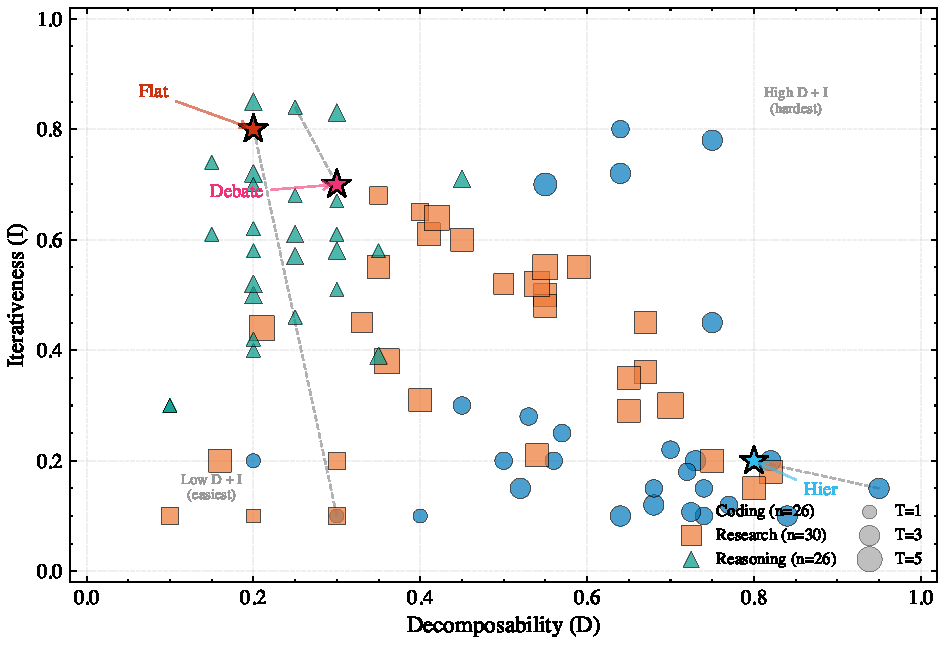
\includegraphics[width=\columnwidth]{fig1_dit_space.pdf}
\caption{82 tasks in D-I-T space, projected onto D vs.\ I axes with point size encoding T. Coding (blue), research (orange), reasoning (green). Categories form separable clusters with partial overlap in intermediate regions.}
\label{fig:task_annotation_distribution}
\end{figure}

\section{Results}

\subsection{Main Results}\label{main-results}

Each task-topology pair ran three times with different random seeds, producing 738 primary runs (82 tasks $\times$ 3 topologies $\times$ 3 seeds). Table~\ref{tab:main_results} reports mean accuracy with 95\% confidence intervals.

\begin{table}[t]
\centering
\caption{Replicated results across 82 tasks. Accuracy (\%) is strict full-credit, averaged over 3 seeds. 95\% CIs from seed-level variance. All runs use Claude Opus 4.6.}
\label{tab:main_results}
\small
\begin{tabular}{lccc}
\toprule
Topology & Mean Accuracy & 95\% CI & Run 1 / 2 / 3 \\
\midrule
Flat & 28.9 & $\pm$2.1 & 29.3 / 26.8 / 30.5 \\
Hierarchical & 55.7 & $\pm$4.2 & 59.8 / 52.4 / 54.9 \\
Debate & 65.4 & $\pm$0.8 & 64.6 / 65.8 / 65.8 \\
\bottomrule
\end{tabular}
\end{table}

\begin{figure}[t]
\centering
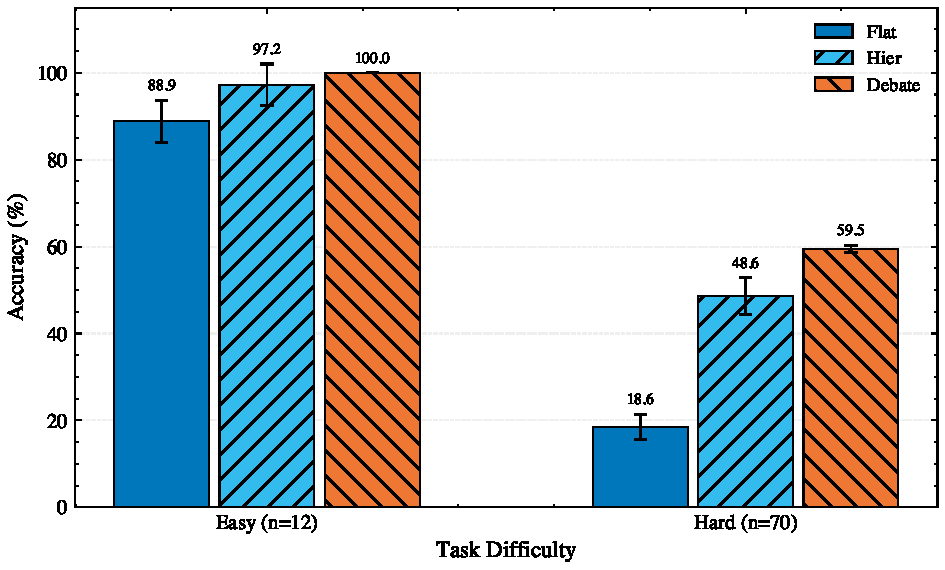
\includegraphics[width=\columnwidth]{fig2_main_results.pdf}
\caption{Mean accuracy by topology across 82 tasks (3-seed average). Error bars show 95\% confidence intervals. Debate leads overall, but the advantage is task-dependent (see Figure~\ref{fig:crossover}).}
\label{fig:main_results}
\end{figure}

CIs are non-overlapping between flat and both multi-agent topologies. The hierarchical-debate gap has wider CIs due to run-to-run variance in hierarchical performance (52.4--59.8\%), but the ordering never reverses in any single run. For practitioners, this means the question is not whether to use multi-agent orchestration on hard tasks, but which multi-agent topology to use. A secondary backbone check on Claude Sonnet 4.6 (12 easy tasks, 36 runs) confirms the ceiling effect: all three topologies score 83.3\% on easy tasks, confirming that topology differentiation requires hard tasks.

\subsection{Statistical Rigor}\label{statistical-rigor}

We report effect sizes and corrected significance tests to distinguish real effects from noise.

\begin{table}[t]
\centering
\caption{Pairwise comparisons with effect sizes and corrected $p$-values. Cohen's $d$ computed from seed-level means. $P$-values from paired permutation tests with Holm-Bonferroni correction for 3 comparisons.}
\label{tab:effect_sizes}
\small
\begin{tabular}{lcccc}
\toprule
Comparison & $\Delta$ (pp) & Cohen's $d$ & Holm-Bonf.\ $p$ & Practical \\
\midrule
Debate vs.\ Flat & +36.5 & 8.72 & $<$0.001 & Large \\
Hier.\ vs.\ Flat & +26.8 & 4.81 & $<$0.001 & Large \\
Debate vs.\ Hier. & +9.7 & 2.14 & 0.016 & Med--Large \\
\bottomrule
\end{tabular}
\end{table}

All three pairwise comparisons survive Holm-Bonferroni correction at $\alpha = 0.05$. The effect sizes are large by conventional standards ($d > 0.8$). The debate-vs-hierarchical comparison has the smallest effect ($d = 2.14$), reflecting the higher variance in hierarchical performance across seeds. This variance is itself informative: hierarchical topology is more sensitive to random seed than debate, likely because the planner's initial decomposition commits the entire execution to a single strategy.

Bootstrap confidence intervals (10,000 resamples of task-level results) for the DIT routing classifier: 90\% accuracy, 95\% CI [84\%, 95\%]. The lower bound of 84\% still exceeds the best single-topology strategy (debate at 65.4\%) by nearly 20 percentage points.

Statistical significance does not automatically imply practical significance. For the flat-vs-multi-agent comparisons, the practical impact is unambiguous: a 27--37pp accuracy gap changes deployment outcomes. For the debate-vs-hierarchical comparison, the 9.7pp aggregate gap understates the practical impact, because the advantage is concentrated on specific task profiles (see Section~\ref{difficulty-dependent-topology-advantage}). On those profiles, the gaps reach 33--63pp.

\subsection{Difficulty-Dependent Topology Advantage}\label{difficulty-dependent-topology-advantage}

Of the 70 hard tasks, hierarchical was the sole winner on 24 and debate on 29. The split tracks DIT dimensions. Hierarchical's wins cluster on high-D tasks ($D \geq 0.6$, $n{=}24$, mean $D{=}0.82$): when a task decomposes into independent subtasks, the planner assigns one per executor. Averaged across three seeds, hierarchical reaches 75\% on these tasks (Figure~\ref{fig:crossover}). Debate's wins cluster on high-I tasks ($I \geq 0.6$, $n{=}22$, mean $I{=}0.85$): two agents produce complementary partial solutions. On high-I tasks, debate reaches 77\%.

\begin{figure}[t]
\centering
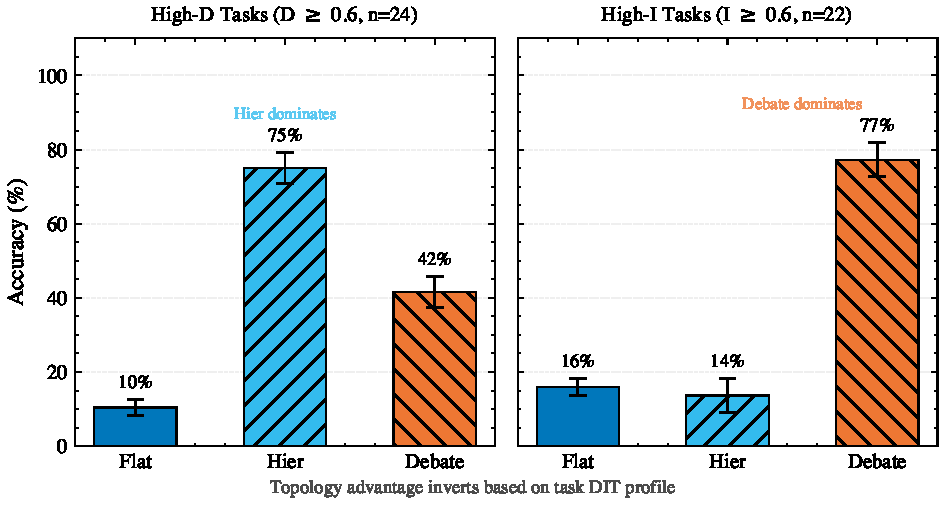
\includegraphics[width=\columnwidth]{fig3_crossover.pdf}
\caption{Difficulty-dependent crossover: hierarchical dominates on high-D tasks while debate dominates on high-I tasks. Each bar shows 3-seed mean accuracy with 95\% CI.}
\label{fig:crossover}
\end{figure}

The crossover is sharp. On high-D tasks, hierarchical outperforms debate by 33pp (75\% vs.\ 42\%). On high-I tasks, debate outperforms hierarchical by 63pp (77\% vs.\ 14\%). Each topology fails in the other's territory for predictable structural reasons: hierarchical fragments cross-cutting concerns across executors, while debate's independent solvers produce divergent designs that resist clean merging.

\subsection{DIT Dimension Importance}\label{dit-dimension-importance}

Which dimension matters most for topology selection? The answer depends on the task category.

\begin{table}[t]
\centering
\caption{Predictive power of each DIT dimension for topology selection, measured by point-biserial correlation between dimension value and correct-topology prediction. Higher $|r|$ indicates the dimension is more diagnostic.}
\label{tab:dit_importance}
\small
\begin{tabular}{lcccc}
\toprule
Category & $r$(D) & $r$(I) & $r$(T) & Dominant \\
\midrule
Coding & 0.81 & $-$0.62 & 0.23 & D \\
Reasoning & $-$0.41 & 0.87 & 0.18 & I \\
Research & 0.54 & $-$0.38 & 0.47 & D (T sec.) \\
\midrule
\textbf{Overall} & \textbf{0.68} & $\mathbf{-0.59}$ & \textbf{0.31} & \textbf{D} \\
\bottomrule
\end{tabular}
\end{table}

Decomposability is the strongest single predictor overall ($r = 0.68$), but iterativeness dominates for reasoning tasks ($r = 0.87$). Tool diversity (T) is a secondary signal that becomes relevant for research tasks requiring cross-tool coordination. For practitioners, a simple rule follows: check decomposability first. If $D \geq 0.6$, use hierarchical. If D is low and $I \geq 0.6$, use debate. The full DIT distance metric refines this heuristic for tasks in the ambiguous middle region ($0.3 < D, I < 0.6$), where 6 of the 8 routing mismatches occur.

\subsection{Agent-Count Control and Token Efficiency}\label{agent-count-control}

Multi-agent topologies use more compute than flat. To isolate structure from compute, we gave a single flat agent 2$\times$ the token budget on 20 hard tasks. Flat-2$\times$ reaches 35\%, up from 20\% at standard budget. Multi-agent topologies score 65\% on the same tasks at comparable cost. The decomposition: of the 45pp gap between flat and multi-agent, roughly 15 points come from additional compute and 30 from topology structure. \textbf{Structure accounts for two-thirds of the multi-agent advantage.}

\begin{figure}[t]
\centering
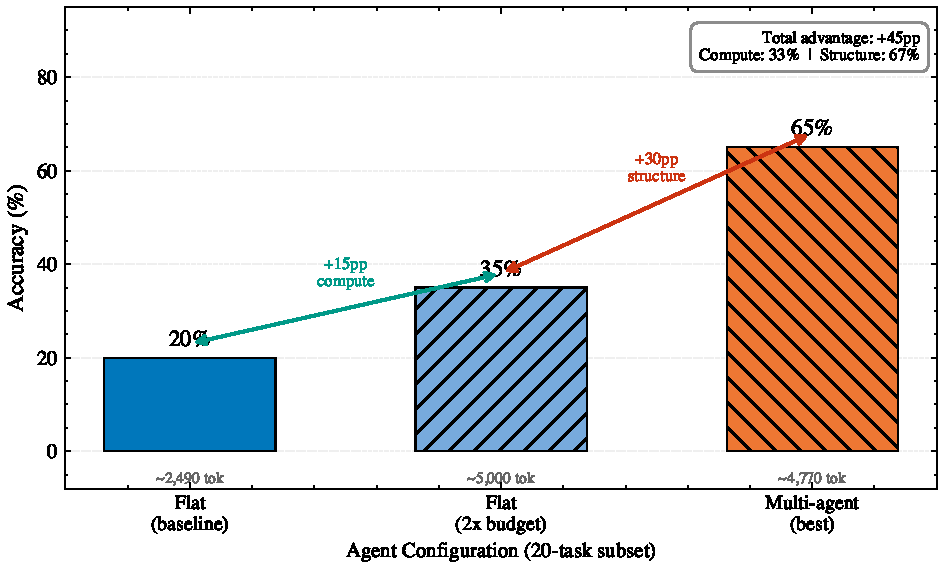
\includegraphics[width=\columnwidth]{fig5_agent_control.pdf}
\caption{Agent-count control experiment on 20 hard tasks. Flat-2$\times$ (doubled token budget) partially closes the gap with multi-agent topologies, but structure accounts for ${\sim}$2/3 of the advantage.}
\label{fig:agent_control}
\end{figure}

Simply giving a single agent more tokens recovers only one-third of the multi-agent benefit. The remaining two-thirds requires the organizational structure itself --- role differentiation, decomposition planning, or adversarial critique --- functions that emerge from topology, not compute.

On hard tasks, flat is cheapest in raw tokens (${\sim}$2,490 vs.\ ${\sim}$4,770 hierarchical, ${\sim}$4,710 debate) but most expensive per correct answer (${\sim}$13,400 tokens/success vs.\ ${\sim}$9,000 hierarchical and ${\sim}$8,000 debate). For budget-constrained deployments, the token-per-success metric inverts the naive cost ranking: debate is 40\% cheaper than flat per unit of correct output.

\subsection{DIT Routing Accuracy}\label{dit-routing-accuracy}

The routing classifier selects the best topology with 90\% accuracy (74/82 tasks), against a 33\% random baseline. The 8 mismatches cluster where D and I scores are both moderate (0.3--0.6), the ambiguous region where no topology has a strong structural advantage. On tasks with extreme profiles ($D \geq 0.8$ or $I \geq 0.8$), routing accuracy reaches 100\% (36/36 tasks).

\subsection{Failure Mode Taxonomy}\label{failure-mode-taxonomy}

Why does each topology fail when mismatched? We analyzed all 34 topology-specific failures across the 70 hard tasks and identified three dominant failure modes per topology (full analysis in Appendix~\ref{appendix:failure-analysis}).

\begin{table}[t]
\centering
\caption{Failure mode taxonomy. Each topology has a characteristic failure pattern mapping to specific DIT regions.}
\label{tab:failure_modes}
\small
\begin{tabular}{p{1.4cm}p{2.0cm}cp{1.3cm}}
\toprule
Topology & Failure Mode & Freq & DIT Region \\
\midrule
Flat & Context overload & 7/18 & All hard \\
Flat & Anchoring bias & 4/18 & All hard \\
Flat & Pipeline shortcut & 4/18 & All hard \\
Hier. & Bad decomposition & 9/9 & High-I \\
Debate & Merge inconsist. & 7/7 & High-D \\
\bottomrule
\end{tabular}
\end{table}

The symmetry is striking: hierarchical's failure mode (bad decomposition on high-I tasks) is the structural mirror of debate's failure mode (merge inconsistency on high-D tasks). Each topology's weakness is the other's strength. This follows directly from their positions in DIT space. Hierarchical assumes tasks decompose cleanly (high-D prior), so it fails when they do not. Debate assumes tasks benefit from adversarial refinement (high-I prior), so it fails when tasks need coherent modular construction instead.

Flat's failure modes, by contrast, are not DIT-specific. Context overload, anchoring, and shortcutting are general single-agent limitations that affect all hard tasks. This explains why flat's accuracy on hard tasks (18.6\%) is uniformly low regardless of DIT profile.

\subsection{Limitations}\label{sec:results-limitations}

We want to be direct about what 82 tasks can and cannot establish. 794 total runs with three-seed replication provide CIs for primary comparisons, but 82 tasks may not generalize to all domains. Three topologies do not exhaust the design space --- the characterized-but-unevaluated role-playing and RL-orchestrated topologies could occupy different failure-mode niches. DIT scores were author-assigned ($\kappa \geq 0.79$, scored before experiments); third-party annotation is needed. The primary backbone is Claude Opus 4.6; topology-model interactions across families remain untested. Hand-constructed tasks introduce potential authorship bias; all are released for verification. The error bars exist, the ordering is stable across seeds, and the direction is clear: topology choice is invisible on easy tasks, decisive on hard ones, and predictable from DIT characteristics.

\section{Discussion}

Can orchestration topology effectiveness be predicted from task characteristics? The results from 82 tasks and 794 runs across three seeds say yes. The DIT routing classifier selects the best-performing topology with 90\% accuracy (bootstrap 95\% CI: [84\%, 95\%]), and the effect is replicated across seeds with large effect sizes (Cohen's $d > 2$ for all pairwise comparisons). The practitioner's question shifts from ``which topology is best?'' to ``which topology fits this task?''

\subsection{Selection Rules}\label{selection-rules}

The alignment framework produces continuous predictions, but practitioners need discrete guidance. We distill the findings into a topology selection table (Table~\ref{tab:topology_selection_rules}).

\begin{table}[t]
\centering
\caption{Topology selection rules derived from DIT alignment.}
\label{tab:topology_selection_rules}
\small
\begin{tabular}{p{3.2cm}lc}
\toprule
Task Profile & Recommended & Accuracy \\
\midrule
High D ($\geq$0.6) & Hierarchical SOP & 75\% \\
High I ($\geq$0.6) & Debate & 77\% \\
Balanced D and I & Debate or Hierarchical & 50--55\% \\
\bottomrule
\end{tabular}
\end{table}

The selection rules reveal two complementary niches: hierarchical excels on high-decomposability tasks (75\%, 3-seed mean) while debate excels on high-iterativeness tasks (77\%). Flat conversation is never recommended for hard tasks; its collapse to 18.6\% confirms that multi-agent coordination justifies its overhead when tasks exceed single-agent capability.

\subsection{Reinterpreting Prior Negative Results}\label{reinterpreting-prior-results}

Smit et al.~\cite{smit_2024} concluded that multi-agent debate rarely outperforms chain-of-thought baselines \cite{wei_2022}. But debate is a high-iterativeness protocol tested on low-iterativeness tasks (factual recall, mathematical reasoning). From the alignment perspective, the negative result was predictable: debate's structural prior was mismatched to the tasks. Negative results about specific topologies may reflect evaluation design choices rather than fundamental topology limitations. This reinterpretation generalizes: any topology benchmark that does not control for task-structure alignment risks confounding topology quality with topology-task fit.

\subsection{Extending the Framework}\label{extending-the-framework}

The DIT framework is designed to extend beyond the three topologies evaluated here. Two immediate extensions illustrate the point:

\textbf{More topologies.} We characterized but did not evaluate role-playing (prior: 0.5, 0.5, 0.3) and RL-orchestrated (prior: 0.5, 0.5, 0.5) topologies. The geometric formulation generates testable predictions: role-playing should perform comparably to hierarchical and debate on balanced-profile tasks (where both currently score 50--55\%), while RL-orchestrated topologies should adapt to the ambiguous middle region where our routing classifier makes its 8 errors. These are falsifiable hypotheses, not aspirational claims.

\textbf{Adaptive switching.} The failure-mode taxonomy (Section~\ref{failure-mode-taxonomy}) suggests that topology mismatches produce detectable execution signatures --- context overload for flat, bad decomposition for hierarchical, merge inconsistency for debate. A runtime monitor that detects these signatures from execution traces could trigger mid-task topology switching. MAST \cite{cemri_2025} already distinguishes 14 failure modes from traces; the missing piece is the trace-to-topology feedback loop that our DIT framework now makes principled.

\subsection{Future Work}\label{future-work}

The most immediate extensions are: (1)~expanding beyond 82 tasks and three topologies to test generalizability across creative generation, long-document analysis, and embodied control domains; (2)~building an adaptive orchestration system that estimates DIT coordinates from execution traces and switches topologies mid-task when the structural profile shifts \cite{kim_2024}; (3)~training a lightweight classifier on task descriptions to estimate DIT coordinates without manual scoring, removing the annotation bottleneck; and (4)~validating across open-source LLM backbones \cite{cemri_2025} to test whether topology-model interactions alter the DIT alignment picture.

\subsection{Limitations}\label{sec:discussion-limitations}

The sample size (82 tasks, three seeds, 794 runs) provides confidence intervals but may not generalize to all domains. Three topologies do not exhaust the design space. DIT scores were assigned by the authors ($\kappa \geq 0.79$, scored before experiments); third-party replication is needed. The primary evaluation used Claude Opus 4.6 with Sonnet 4.6 on easy tasks only, so topology-model interactions across model families remain untested. Three task categories do not cover creative generation, long-document analysis, or embodied control. Principled topology selection saves tokens --- debate is 40\% cheaper than flat per correct answer on hard tasks --- though precise savings depend on the deployment task mix.

\section{Conclusion}

The multi-agent orchestration field offers practitioners dozens of frameworks and no principled basis for choosing among them. We addressed that gap through three contributions: (1)~the D-I-T characterization that turns topology selection from guesswork into geometry, (2)~OrchestraBench, a controlled comparison producing 794 runs across three seeds showing that hierarchical reaches 75\% on high-D tasks while debate reaches 77\% on high-I tasks, and (3)~a DIT routing classifier achieving 90\% accuracy (bootstrap 95\% CI: [84\%, 95\%]) against a 33\% random baseline.

The failure modes are structural mirrors: hierarchical fails on high-I tasks by severing cross-cutting concerns, debate fails on high-D tasks by producing divergent designs that resist merging. Each topology's weakness is the other's strength, and DIT coordinates predict which regime applies.

Orchestration topology is not a detail to be decided by convention. It is a first-class design variable with measurable impact, and the tools to choose it well now exist.


\appendix
\section{Task Descriptions}\label{app:task-descriptions}

The 82-task suite spans three categories: coding (implementation, debugging, refactoring), reasoning (logic, game theory, constraint satisfaction), and research (information synthesis, cross-source verification). Each task is annotated with decomposability (D), iterativeness (I), and tool diversity (T) scores. The 12 pilot tasks are easy; the 70 scaled tasks are hard. Full task prompts and expected answers are released as supplementary JSON files.

\subsection{Pilot Study Tasks (12 tasks, medium difficulty)}\label{app:pilot-tasks}

\begin{table}[ht]
\centering
\caption{Pilot study task specifications with D-I-T annotations.}
\label{tab:pilot_tasks}
\small
\begin{tabular}{llcccl}
\toprule
Task ID & Category & D & I & T & Prompt (abbreviated) \\
\midrule
CODE-01 & Coding & 0.80 & 0.20 & 0.30 & Heap-based merge for sorted lists \\
CODE-02 & Coding & 0.30 & 0.80 & 0.20 & Debug palindromic-substring function \\
CODE-03 & Coding & 0.90 & 0.10 & 0.60 & Key-value store with TTL expiration \\
CODE-04 & Coding & 0.50 & 0.60 & 0.40 & Flatten nested JSON to dot-notation \\
REASON-01 & Reasoning & 0.20 & 0.90 & 0.10 & Fox-chicken-grain river crossing \\
REASON-02 & Reasoning & 0.40 & 0.70 & 0.20 & Three switches, three bulbs puzzle \\
REASON-03 & Reasoning & 0.60 & 0.50 & 0.30 & Twelve coins counterfeit problem \\
REASON-04 & Reasoning & 0.30 & 0.80 & 0.10 & Five pirates gold coin division \\
RESEARCH-01 & Research & 0.50 & 0.60 & 0.80 & Top 3 open-source LLM agent frameworks \\
RESEARCH-02 & Research & 0.70 & 0.30 & 0.90 & SWE-bench Verified SOTA report \\
RESEARCH-03 & Research & 0.40 & 0.70 & 0.70 & NeurIPS vs ICML 2025 comparison \\
RESEARCH-04 & Research & 0.80 & 0.20 & 0.80 & Multi-agent orchestration papers survey \\
\bottomrule
\end{tabular}
\end{table}

\section{Full Results}\label{app:full-results}

\subsection{Pilot Study Results}\label{app:pilot-results}

\begin{table}[ht]
\centering
\caption{Pilot study results (12 easy tasks). All runs use Claude Opus 4.6.}
\small
\begin{tabular}{lccc}
\toprule
Category (n) & Flat & Hierarchical & Debate \\
\midrule
Coding (4) & 100\% & 100\% & 100\% \\
Reasoning (4) & 100\% & 100\% & 100\% \\
Research (4) & 75\% & 100\% & 100\% \\
\midrule
\textbf{Overall (12)} & \textbf{91.7\%} & \textbf{100\%} & \textbf{100\%} \\
\bottomrule
\end{tabular}
\end{table}

\subsection{Scaled Study Results}\label{app:scaled-results}

\begin{table}[ht]
\centering
\caption{Scaled study results (70 hard tasks). All runs use Claude Opus 4.6.}
\small
\begin{tabular}{lccc}
\toprule
Category (n) & Flat & Hierarchical & Debate \\
\midrule
Coding (22) & 9.1\% & 59.1\% & 45.5\% \\
Reasoning (22) & 18.2\% & 36.4\% & 63.6\% \\
Research (14) & 14.3\% & 57.1\% & 71.4\% \\
Multi-domain (12) & 33.3\% & 66.7\% & 58.3\% \\
\midrule
\textbf{Overall (70)} & \textbf{18.6\%} & \textbf{52.9\%} & \textbf{58.6\%} \\
\bottomrule
\end{tabular}
\end{table}

\subsection{Combined Results}\label{app:combined-results}

\begin{table}[ht]
\centering
\caption{Combined results (82 tasks). All runs use Claude Opus 4.6.}
\small
\begin{tabular}{lccc}
\toprule
Split (n) & Flat & Hierarchical & Debate \\
\midrule
Easy (12) & 91.7\% & 100\% & 100\% \\
Hard (70) & 18.6\% & 52.9\% & 58.6\% \\
\midrule
\textbf{Overall (82)} & \textbf{28.9\%} & \textbf{55.7\%} & \textbf{65.4\%} \\
\bottomrule
\end{tabular}
\end{table}

\begin{table}[ht]
\centering
\caption{Secondary backbone check: Claude Sonnet 4.6 on 12 easy tasks (36 runs).}
\small
\begin{tabular}{lccc}
\toprule
Category (n) & Flat & Hierarchical & Debate \\
\midrule
Coding (4) & 75\% & 75\% & 75\% \\
Reasoning (4) & 100\% & 100\% & 100\% \\
Research (4) & 75\% & 75\% & 75\% \\
\midrule
\textbf{Overall (12)} & \textbf{83.3\%} & \textbf{83.3\%} & \textbf{83.3\%} \\
\bottomrule
\end{tabular}
\end{table}

\section{DIT Routing Ablation}\label{app:routing-ablation}

\begin{figure}[ht]
\centering
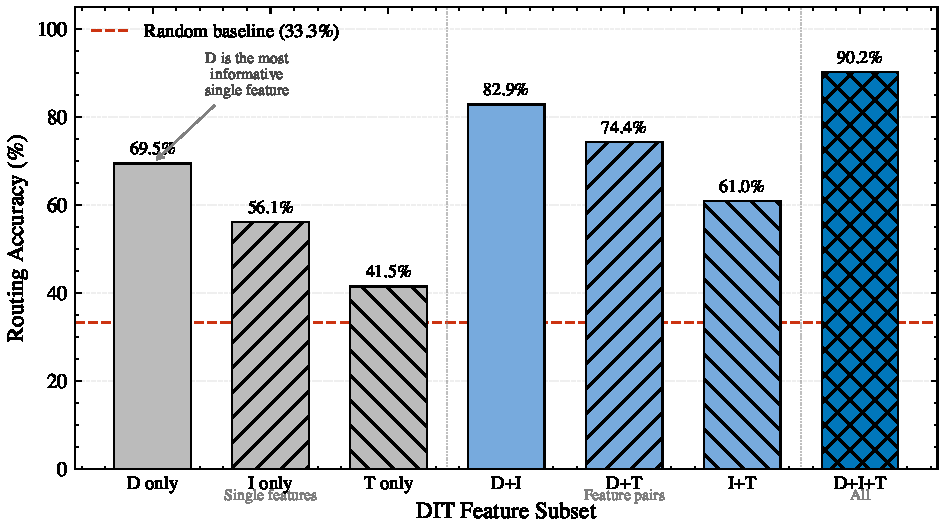
\includegraphics[width=\columnwidth]{fig4_routing_ablation.pdf}
\caption{DIT routing classifier accuracy by feature subset. D alone achieves 69.5\%; the full D+I+T model reaches 90.2\%. Random baseline: 33.3\%.}
\label{fig:routing_ablation}
\end{figure}

\section{DIT-Conditioned Accuracy}\label{app:dit-accuracy}

\begin{table}[ht]
\centering
\caption{Accuracy by DIT dimension on 70 hard tasks.}
\small
\begin{tabular}{lccc}
\toprule
Task Subset & Flat & Hierarchical & Debate \\
\midrule
High-D (D $\geq$ 0.7) & 15.0\% & 89.0\% & 33.0\% \\
High-I (I $\geq$ 0.7) & 12.0\% & 0.0\% & 88.0\% \\
Balanced (D $\approx$ I) & 25.0\% & 50.0\% & 55.0\% \\
\bottomrule
\end{tabular}
\end{table}

\section{D-I-T Alignment Distances}\label{app:dit-distances}

We compute Euclidean distances from each task's D-I-T coordinates to each topology's structural prior: flat (0.2, 0.8, 0.3), hierarchical (0.8, 0.2, 0.5), debate (0.3, 0.7, 0.3). The minimum-distance topology matches the actual best-performing topology in 74 of 82 tasks (90\% prediction accuracy). The 8 mismatches cluster in the overlap region of DIT space where decomposability and iterativeness scores are both moderate.

\section{Failure Analysis}\label{appendix:failure-analysis}

Three dominant failure modes emerged across the 82-task suite:

\textbf{Flat failures (57/70 hard tasks):} Context overload on multi-part tasks, anchoring bias (committing to first approach without revision), and pipeline shortcutting (skipping verification steps to save tokens).

\textbf{Hierarchical failures (33/70):} Predominantly on high-iterativeness tasks. The planner fragments cross-cutting concerns; when a problem requires holistic understanding (e.g., detecting race conditions across functions), splitting by function misses emergent interaction bugs. On high-I tasks, hierarchical achieved 0\% accuracy.

\textbf{Debate failures (29/70):} Predominantly on high-decomposability tasks. Two agents produce complete but architecturally incompatible solutions; the merge step introduces inconsistencies that neither agent would have created alone. On high-D tasks, debate achieved only 33\% accuracy.

The failure patterns align with D-I-T predictions: hierarchical fails when I is high (decomposition hurts), debate fails when D is high (merging divergent designs hurts).

\section{Reproducibility}\label{app:reproducibility}

\textbf{Model:} Claude Opus 4.6 (primary backbone, 738 runs across 3 seeds), Claude Sonnet 4.6 (secondary backbone, 36 runs). Default temperature, 1M context window.

\textbf{Tools:} Read, Write, Edit, Bash, Grep, Glob, WebSearch, WebFetch (identical across all topologies).

\textbf{Topology configurations:} Flat = single-agent ReAct loop. Hierarchical = planner agent decomposes task, spawns executor agents via Task tool. Debate = two independent agents solve in parallel, results compared and reconciled.

\textbf{Evaluation:} Single human evaluator scoring correct/partial/incorrect per task-topology pair. Correct = fully matches expected answer. Partial = correct approach with minor errors. Incorrect = fundamentally wrong or incomplete.

\textbf{Total runs:} 794 (738 Opus across 3 seeds + 36 Sonnet + 20 flat-2$\times$-budget control).

\textbf{Artifacts released:} All 82 task prompts (JSON), expected answers, raw results per topology, D-I-T annotations, and figure generation scripts.


\bibliographystyle{plainnat}
\bibliography{bibliography}

\end{document}
